%!TEX root = ../thesis.tex
%*******************************************************************************
%****************************** Third Chapter **********************************
%*******************************************************************************
\chapter{Σχήματα και Πίνακες}

% **************************** Define Graphics Path **************************
\ifpdf
    \graphicspath{{Chapter3/Figs/Raster/}{Chapter3/Figs/PDF/}{Chapter3/Figs/}}
\else
    \graphicspath{{Chapter3/Figs/Vector/}{Chapter3/Figs/}}
\fi
\begin{figure}[htbp!] 
\centering    
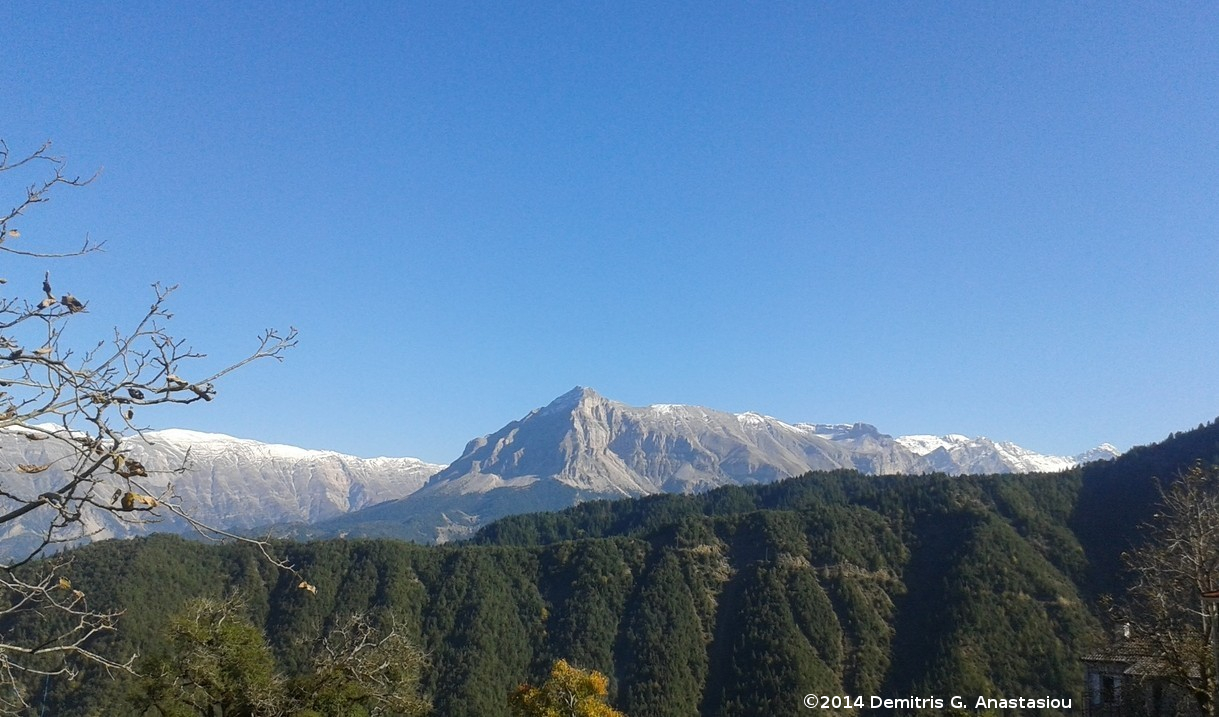
\includegraphics[width=\textwidth]{back-skloupo1.jpg}
\bicaption[Σκλούπο-Στρογγούλα]{Από το χωριό Σκλούπο\index{Σκλούπο}  η θέα προς τη Στρογγούλα\index{Στρογγούλα}(2374μ) στα Τζουμέρκα\index{Τζουμέρκα}.}{The view towards Stroggoula mountain (2374m) in Tzoumerka, from my village Skloupo!! }
\label{fig:minion}
\end{figure} 


%\addtocounter{footnote}{-3} %3=n
%\stepcounter{footnote}
\footnotetext{Σκλούπο: φ: 39$^\circ$ 31' 42''.74 λ: 21$^\circ$ 01' 48".92}
%\stepcounter{footnote}
\footnotetext{Στρογγούλα: φ: 39$^\circ$ 29' 48''.98 λ: 21$^\circ$ 07' 02".32}

\clearpage
\section{Εισαγωγή Σχημάτων στο κείμενο}

\begin{figure}[htbp!] 
\centering    

\includegraphics[width=\textwidth]{minion}
\bicaption[Συμπτηγμένη λεζάντα]{Αυτή είναι μία λεζάντα\index{λεζάντα} μεγάλη για την οποία μπορούμε να χρησιμοποιηθεί και μια μικρότερη έκδοση.}{This is just a long figure caption for the minion in Despicable Me from Pixar}
\label{fig:minion}
\end{figure}

\begin{landscape}

\section*{Subplots}
I can cite Wall-E (see Fig.~\ref{fig:WallE}) and Minions in despicable me (Fig.~\ref{fig:Minnion}) or I can cite the whole figure as Fig.~\ref{fig:animations}


\begin{figure}
  \centering
  \begin{subfigure}[b]{0.3\textwidth}
    
\includegraphics[width=\textwidth]{TomandJerry}
    \caption{Tom and Jerry}
    \label{fig:TomJerry}   
  \end{subfigure}             
  \begin{subfigure}[b]{0.3\textwidth}
    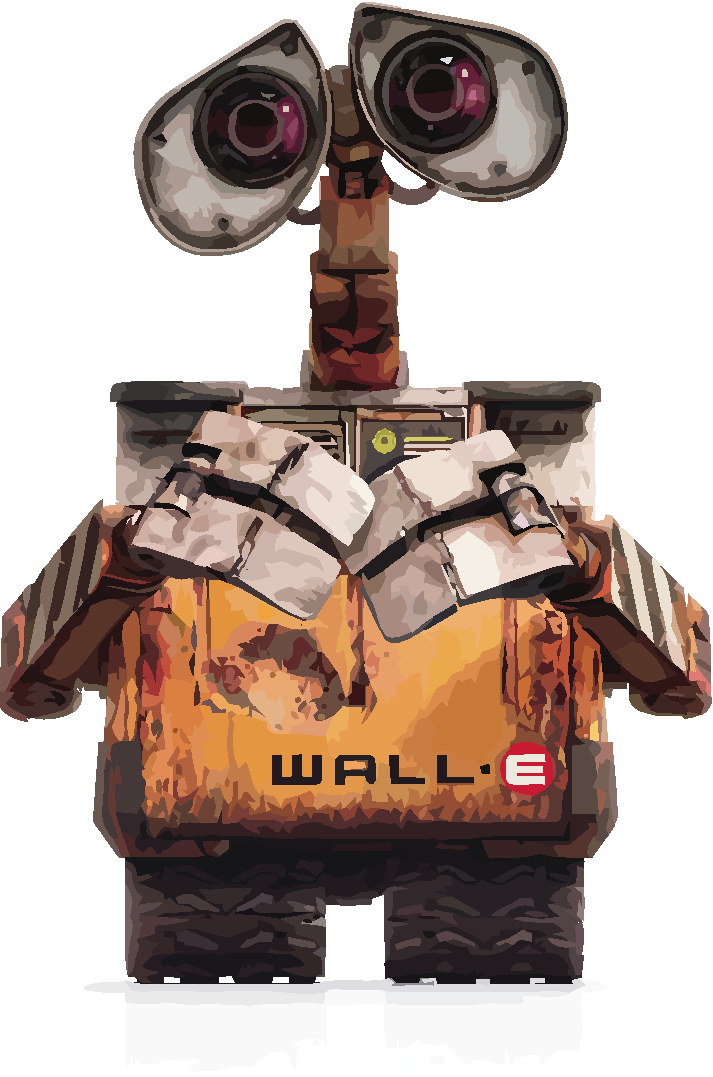
\includegraphics[width=\textwidth]{WallE}
    \caption{Wall-E}
    \label{fig:WallE}
  \end{subfigure}             
  \begin{subfigure}[b]{0.3\textwidth}
    
\includegraphics[width=\textwidth]{minion}
    \caption{Minions}
    \label{fig:Minnion}
  \end{subfigure}
  \bicaption{Τα καλύτερα κινούμενα σχέδια}{Best Animations}
  \label{fig:animations}
\end{figure}


\end{landscape}



\section{Διαμόρφωση Πινάκων}

Το παρόν κεφάλαιο έχει διαμορφωθεί με βάση το ``Publication quality tables in \LaTeX*''
 από τον Simon Fear. Αφήνω επομένως τις οδηγίες όπως ειναι στο πρωτότυπο κείμενο.

The layout of a table has been established over centuries of experience and 
should only be altered in extraordinary circumstances. 

When formatting a table, remember two simple guidelines at all times:

\begin{enumerate}
  \item Never, ever use vertical rules (lines).
  \item Never use double rules.
\end{enumerate}

These guidelines may seem extreme but I have
never found a good argument in favour of breaking them. For
example, if you feel that the information in the left half of
a table is so different from that on the right that it needs
to be separated by a vertical line, then you should use two
tables instead. Not everyone follows the second guideline:

There are three further guidelines worth mentioning here as they
are generally not known outside the circle of professional
typesetters and subeditors:

\begin{enumerate}\setcounter{enumi}{2}
  \item Put the units in the column heading (not in the body of
          the table).
  \item Always precede a decimal point by a digit; thus 0.1
      {\em not} just .1.
  \item Do not use `ditto' signs or any other such convention to
      repeat a previous value. In many circumstances a blank
      will serve just as well. If it won't, then repeat the value.
\end{enumerate}

A frequently seen mistake is to use `\textbackslash begin\{center\}' \dots `\textbackslash end\{center\}' inside a figure or table environment. This center environment can cause additional vertical space. If you want to avoid that just use `\textbackslash centering'


\begin{table}
\bicaption{Ένας κακά διαμορφωμένος πίνακας}{A badly formatted table}
\centering
\label{table:bad_table}
\begin{tabular}{|l|c|c|c|c|}
\hline 
& \multicolumn{2}{c}{Species I} & \multicolumn{2}{c|}{Species II} \\ 
\hline
Dental measurement  & mean & SD  & mean & SD  \\ \hline 
\hline
I1MD & 6.23 & 0.91 & 5.2  & 0.7  \\
\hline 
I1LL & 7.48 & 0.56 & 8.7  & 0.71 \\
\hline 
I2MD & 3.99 & 0.63 & 4.22 & 0.54 \\
\hline 
I2LL & 6.81 & 0.02 & 6.66 & 0.01 \\
\hline 
CMD & 13.47 & 0.09 & 10.55 & 0.05 \\
\hline 
CBL & 11.88 & 0.05 & 13.11 & 0.04\\ 
\hline 
\end{tabular}
\end{table}

\begin{table}
\bicaption{Ένας όμορφα διαμορφωμένος πίνακας}{A nice looking table}
\centering
\label{table:nice_table}
\begin{tabular}{l c c c c}
\hline 
\multirow{2}{*}{Dental measurement} & \multicolumn{2}{c}{Species I} & \multicolumn{2}{c}{Species II} \\ 
\cline{2-5}
  & mean & SD  & mean & SD  \\ 
\hline
I1MD & 6.23 & 0.91 & 5.2  & 0.7  \\

I1LL & 7.48 & 0.56 & 8.7  & 0.71 \\

I2MD & 3.99 & 0.63 & 4.22 & 0.54 \\

I2LL & 6.81 & 0.02 & 6.66 & 0.01 \\

CMD & 13.47 & 0.09 & 10.55 & 0.05 \\

CBL & 11.88 & 0.05 & 13.11 & 0.04\\ 
\hline 
\end{tabular}
\end{table}


\begin{table}
\bicaption{Ο πιο σωστά διαμορφωμένος πίνακας}{Even better looking table using booktabs}
\centering
\label{table:good_table}
\begin{tabular}{l c c c c}
\toprule
\multirow{2}{*}{Dental measurement} & \multicolumn{2}{c}{Species I} & \multicolumn{2}{c}{Species II} \\ 
\cmidrule{2-5}
  & mean & SD  & mean & SD  \\ 
\midrule
I1MD & 6.23 & 0.91 & 5.2  & 0.7  \\

I1LL & 7.48 & 0.56 & 8.7  & 0.71 \\

I2MD & 3.99 & 0.63 & 4.22 & 0.54 \\

I2LL & 6.81 & 0.02 & 6.66 & 0.01 \\

CMD & 13.47 & 0.09 & 10.55 & 0.05 \\

CBL & 11.88 & 0.05 & 13.11 & 0.04\\ 
\bottomrule
\end{tabular}
\end{table}

\clearpage
\begin{longtabu} to \textwidth {r || *{8}{X}}

%This is the Κωδικός  & & \multicolumn{3}{c}{diffs} \\ for the first page of the table...
%    \caption{Χρονικές περίοδοι μετρήσεων στο δίκτυου 1ης τάξης. }
\bicaption{Πίνακας που συνεχίζεται και σε επόμενη σελίδα.}{The table continuous on the next page.}
   \label{tab:epochstr}\\
 
    \toprule
    % Header for the first page of the table
    Κωδικός & \multicolumn{8}{c}{Χρονική περίοδος των παρατηρήσεων}\\
    Τριγώνου & \\
    \midrule
    \endfirsthead


    %This is the header for the remaining page(s) of the table...
    \multicolumn{9}{l}{\textit{(Συνέχεια από την προηγούμενη σελίδα \ldots)}}\\
    \toprule
    Κωδικός & \multicolumn{8}{c}{Χρονική περίοδος των παρατηρήσεων}\\
    Τριγώνου & \\
    \midrule
    \endhead
    
    %This is the footer for all pages except the last page of the table...
    \bottomrule
    \multicolumn{9}{r}{\textit{(Συνεχίζεται στην επόμενη σελίδα \ldots)}}\\
    \endfoot
    
    %This is the footer for the last page of the table...
    \bottomrule
    \endlastfoot
    
062 & & 1940 & 1959 & 1964\\
063 & 9010 & 1940 & 1957 & 1964 & 1965\\
064 & 9010 & 1940 & 1954 & 1964 & 1965 & 1966\\
066 & & 1940 & 1959 & 1964 & 1965 \\
070 & 9010 & 1940 & 1952 & 1967 & 1976\\
071 & 9010 & 1940 & 1958 & 1976 & 1983\\
072 & 9010 & 1940 & 1965 & 1967 & 1980\\
075 & 9010 & 1940 & 1976\\
076 & 9010 & 1940 & 1952 & 1967 & 1969 & 1976\\
077 & 9010 & 1940 & 1967 & 1969 & 1976 & 1982\\
078 & 9010 & 1940 & 1968 & 1969 & 1975 & 1982\\
089 & & 1940 & 1968 & 1969 & 1976 & 1983\\
090 & & 1940 & 1968 & 1969 & 1975 & 1976 & 1983\\
091 & & & 1953 & 1965 & 1976\\
092 & 9010 & 1940 & 1954 & 1963 & 1965 & 1966 & 1976 & 1983\\
093 & 9010 & 1940 & 1954 & 1965\\
094 & 9010 & 1940 & 1955 & 1965 & 1966 & 1983\\
095 & & & 1954 & 1956 & 1965\\
096 & & & 1954 & 1965\\
097 & & & 1954 & 1965\\
098 & 9010 & 1940 & 1953 & 1956 & 1983\\
099 & 9010 & 1940 & 1953 & 1969\\
100 & 9010 & 1940 & 1953 & 1969 & 1980\\
101 & 9010 & 1940 & 1952 & 1969 & 1976 & 1983\\
102 & & 1940 & 1952 & 1956 & 1968 & 1969 & 1976\\
103 & & 1940 & 1958 & 1964\\
104 & 9010 & 1940 & 1958 & 1959 & 1964\\
105 & 9010 & 1940 & 1958 & 1959 & 1964 & 1977 & 1984\\
106 & 9010 & 1940 & 1958 & 1959 & 1977 & 1984\\
107 & 9010 & 1940 & 1958 & 1959 & 1977 & 1984\\
108 & 9010 & 1940 & 1959 & 1984\\
109 & 9010 & 1940 & 1958 & 1959 & 1965\\
110 & 9010 & 1940 & 1956 & 1965\\
111 & 9010 & 1940 & 1959 & 1965 & 1984\\
112 & & 1940 & 1954 & 1956 & 1976 & 1982\\
113 & 9010 & 1940 & 1956 & 1976 & 1982\\
114 & 9010 & 1940 & 1956 & 1976 & 1982\\
115 & 9010 & 1940 & 1956 & 1976 & 1982\\
116 & & 1940 & 1952 & 1956 & 1976 & 1982\\
117 & & 1940 & 1952 & 1954 & 1956 & 1976 & 1982\\
120 & & 1940 & 1956 & 1968 & 1972 & 1975 & 1976 & 1983\\
121 & 9010 & 1940 & 1956 & 1972 & 1976 & 1982\\
136 & & & 1954 & 1956 & 1970 & 1983\\
145 & 9010 & 1940 & 1957 & 1970\\
146 & 9010 & 1940 & 1959\\
147 & 9010 & 1940 & 1960\\
149 & 9010 & 1940 & 1959 & 1977\\
150 & 9010 & 1940 & 1959 & 1977\\
151 & & & 1959 & 1977\\
152 & & & 1959 & 1977 & 1986\\
153 & & & 1959 & 1981\\
154 & & & 1959 & 1977 & 1986\\
155 & & & 1959 & 1977 & 1986\\
156 & & & 1959 & 1977\\
157 & 9010 & 1940 & 1959 & 1960 & 1986\\
158 & & & 1959 & 1960 & 1977 & 1986\\

\end{longtabu}
